\documentclass[conference]{IEEEtran}
\usepackage[utf8]{inputenc}
\usepackage{url}
\usepackage{amsmath}
\usepackage{amssymb}
\usepackage{graphicx}
\usepackage[colorlinks=true, linkcolor=blue, citecolor=blue, urlcolor=blue]{hyperref}


\begin{document}

\title{Seminar - Collective navigation of a multi-robot system in an unknown environment}
\author{\IEEEauthorblockN{Gregor Germerodt}
\IEEEauthorblockA{Hochschule Trier - Trier University of Applied Sciences\\
E-Mail: grgr3403@hochschule-trier.de\\
Themensteller und Betreuer: Prof. Dr. Jürgen Graf\\
Cognitive Systems and Robotics}}

\maketitle


\begin{abstract}
This paper is a summary of the work of Olcay (2020). 
All content is based on this work and its referenced sources have been 
incorporated where necessary.

Various methods for the movement of robots in unknown environments are presented,
for collision avoidance and target achievement using virtual forces. First, the methods
for a single robot are explained and then extended to a multi-robot system with the 
help of a communication network.
\end{abstract}

\section{Introduction}
\cite{Olcay.2020} Multi-robot systems, such as autonomous robots collaborating in a swarm, 
offer applications in unknown environments like mapping, exploration, or 
rescue missions \cite{Stormont.null}. 
To ensure collision-free paths, this work addresses 
collective navigation under limited sensor and communication ranges. To 
enhance system robustness, a nature-inspired swarm behavior is applied, 
based on three simple rules: cohesion, separation, and alignment 
\cite{Reynolds.1987}. 
While global motion planning assumes an initial map with static obstacles, 
this work focuses on local motion planning that can dynamically respond 
to environmental changes. Instead of using Simultaneous Localization and 
Mapping (SLAM), where robots build a map while estimating their own 
position, this approach relies on a decentralized, potential field-based 
navigation method using only local sensor data and neighbor-to-neighbor 
communication. This enables the robots to make early, collective decisions 
for collision avoidance while ensuring scalability and flexibility of 
the system.

\section{Theoretical background}
In the multi-robot system under consideration, the robots are modeled as point masses 
(i.e., without spatial extension, only by position and mass point) in a 
two-dimensional environment. The system dynamics are based on potential field-based 
forces, whereby only the position and velocity of each robot $i$ are taken into account,
$(p_i, v_i) \in \mathbb{R}^2 \times \mathbb{R}^2$.
The motion dynamics of each robot $i$ are described by the following differential equations:
\begin{equation}
    \dot{p}_i = v_i
    \label{eq:1}
\end{equation}
\begin{equation}
    \dot{v}_i = u_i
    \label{eq:2}
\end{equation}
The position of the robot therefore changes with its velocity \eqref{eq:1}, which in turn changes 
due to a control force \eqref{eq:2}.
Each robot can only interact bidirectionally with neighboring robots within a fixed 
communication radius $r_c$. The time-dependent and undirected 
neighborhood is defined by
\begin{equation}
    \mathcal{N}_i^\alpha = \{ j \in \mathcal{V} \; | \; \| p_j - p_i \| < r_c \}
    \label{eq:3}
\end{equation}
with $\mathcal{V} = \{1, \ldots, N\},\ N \in \mathbb{N}$, the set of all robots.
To generate swarm behavior, distance values are calculated between two robots, 
which determine the deviation energy, the degree of interaction, and connectedness 
(\eqref{eq:16} to \eqref{eq:18}).

The control force $u_i$ of a robot $i$ is calculated using the equation
\begin{equation}
    u_i = u_i^\alpha + u_i^\beta + u_i^\gamma
    \label{eq:4}
\end{equation}
where $u_i^\alpha$ is for swarm behavior, $u_i^\beta$ is for 
obstacle avoidance, and $u_i^\gamma$ for navigation. The swarm behavior 
$u_i^\alpha$ consists of distance and speed adjustments to neighbors 
(\eqref{eq:19}) 
and their effectiveness depending on the distance 
(\eqref{eq:20} to \eqref{eq:21}).

Obstacle avoidance $u_i^\beta$ is defined by the obstacle points 
detected by a robot (\eqref{eq:22}), how strongly it is repelled by them 
(\eqref{eq:23}) and how this repulsive force is calculated as a equation of distance 
(\eqref{eq:24}). The control force for navigation $u_i^\gamma$ 
attracts the robot to the target (\eqref{eq:25}).


\subsection*{The problem statement}
Many existing navigation approaches for multi-robot systems are based on artificial 
potential fields, in which robots are attracted to target points and repelled by obstacles. However, a central problem with these methods is local minima, in which 
attractive and repulsive forces balance each other out and robots get stuck. 

Methods for individual robots, such as camera- or elimination-based approaches, reach their limits in 
difficult environmental conditions or obstacle configurations.

Furthermore, the challenge for multi-robot systems is to navigate collision-free and 
efficiently in unknown and complex environments, despite limited 
sensor and communication ranges. 
For this reason, this study deals with communication and motion planning 
for multiple robots,
whereby noise effects, time delays or packet loss are not taken into account.


\section{Single robot navigation}
\label{sec:Single robot navigation}
Before a robot can act in a swarm, it must be able to cope on its own. Three methods are presented in this section:
\begin{itemize}
    \item Tangential navigation, inspired by \cite{Brandao.2013},
    \item Corner avoidance, and
    \item Motion planning at obstacle extremities.
\end{itemize}

Basically, a robot wants to move to a specified destination while watching out for obstacles within a certain sensor radius \(r_{\mathrm{tan}}\). If it detects an obstacle (represented by the point \( \hat{p}_{i,k} \)), it avoids it by moving parallel to the edge of the obstacle, i.e., tangentially.
This is done taking into account the angles \( \alpha_i \) and \( \beta_i \) depending on the direction of movement and the resulting rotation angle \( \gamma_i \). 
These angles determine the evasion direction 
(\eqref{eq:26} to \eqref{eq:28}) and a virtual goal 
(\eqref{eq:29}). Using an adjusted control force 
(\eqref{eq:30} similar to \eqref{eq:25}),
 the robot is accelerated toward the virtual goal $p_i^v$.

\begin{figure}[h]
    \centering
    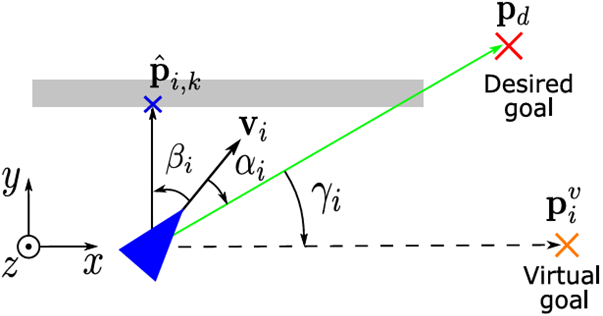
\includegraphics[width=0.4\textwidth]{Pictures/Strategy for tangential navigation.png}
    \caption{Strategy for tangential navigation.}
    \label{fig:Strategy for tangential navigation}
\end{figure}

If the robot detects two obstacles (represented by two points \( \hat{p}_{i,n} \) and \( \hat{p}_{i,n90} \)) 
that form a corner, it applies the \textit{Corner Avoidance} maneuver. 
In this maneuver, the rotation angle \( \gamma_i \) is supplemented by an additional angle \( \varepsilon_i \),
 which is calculated from the tangent directions $n$ and $n_{90}$ to both obstacle points 
relative to the robot 
(\eqref{eq:31} to \eqref{eq:32}). Then,
a virtual goal $p_i^v$ is determined again, which guides the robot out of the corner (\eqref{eq:33}).

\begin{figure}[h]
    \centering
    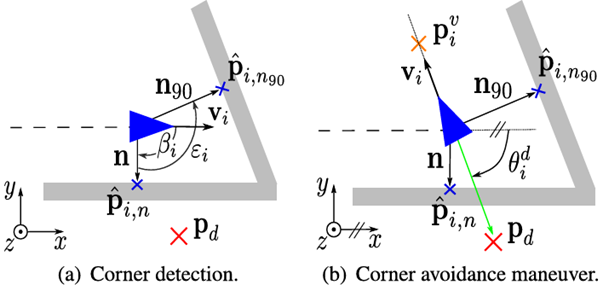
\includegraphics[width=0.4\textwidth]{Pictures/Strategy for corner avoidance.png}
    \caption{Strategy for corner avoidance.}
    \label{fig:Strategy for corner avoidance}
\end{figure}

When the robot reaches the end of an obstacle, it performs a 
circular movement around the end. To do this, it remembers the last 
obstacle point \( \hat{p}_{i,e} \) that was registered within its sensor radius. Using  
equation \eqref{eq:34} and the angle \( \beta_{i} \), which was obtained by tangential navigation,
 the robot calculates virtual goals at equal intervals (calculated 
by equation \eqref{eq:35} and represented by the points \( p_i^{v1} \), 
\( p_i^{v2} \) and \( p_d \)) at equal intervals and rotates by a 
fixed angle \( \delta \) until the angle between the motion vector and the virtual 
target is less than or equal to \( \delta \) (\eqref{eq:36}).

\begin{figure}[h]
    \centering
    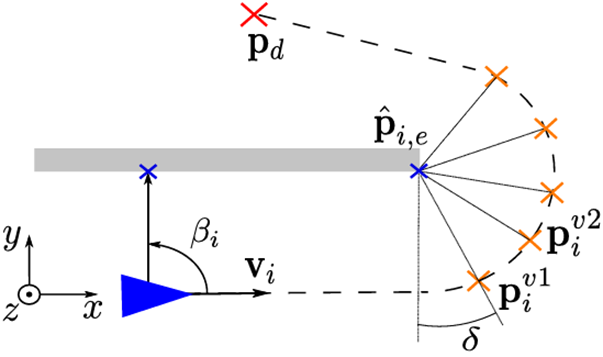
\includegraphics[width=0.4\textwidth]{Pictures/Circular Motion at obstacle endpoint.png}
    \caption{Circular Motion at obstacle endpoint.}
    \label{fig:Circular Motion at obstacle endpoint}
\end{figure}


\section{The proposed navigation approach for a multi-robot system}
The approach presented here extends the navigation algorithm for individual robots 
with a communication interface for the collective motion planning of multiple 
robots. The cohesion of the group could be at risk if each robot 
pursues its own virtual goal. Therefore, information about virtual 
targets and critical points 
(as shown in Fig.~\ref{fig:The critical points of obstacles}) is exchanged between them. 
This information is prioritized according to relevance, timeliness, and the principle of "detection before 
communication" (detected obstacles take precedence over transmitted 
information from the communication network).
The communication network consists of information packages, which are divided into three types
: orientation, endpoints, and corners.

\begin{figure}[h]
    \centering
    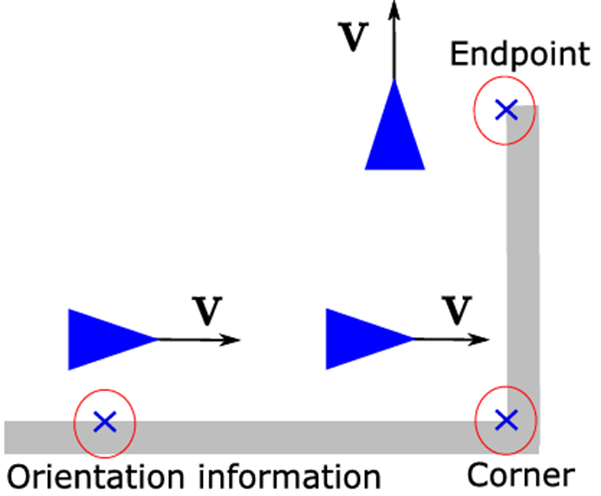
\includegraphics[width=0.25\textwidth]{Pictures/The critical points of obstacles.png}
    \caption{The critical points of obstacles.}
    \label{fig:The critical points of obstacles}
\end{figure}

\textbf{Orientation (Fig.~\ref{fig:Information about orientation}):} 
Contains the angle \( \theta_i \) to the current target, the detected 
point \( \hat{p}_{i,k} \) on the obstacle, the current status of the 
robot (all statuses explained in \ref{tab:status}) and the time of obstacle detection.

\textbf{Endpoints (Fig.~\ref{fig:Endpoint and corner Information} (a)):} 
Consists of the last detected point \( \hat{p}_{i,e} \), the angle \( \omega_{i,e} \) 
between the normal vector from the robot to the obstacle and the x-axis of the inertial 
coordinate system\footnote{unaccelerated and subject to the law of inertia 
coordinate system} and the target angle \( \theta_{i,e} \) at the moment of endpoint detection.

\textbf{Corners (Fig.~\ref{fig:Endpoint and corner Information} (b)):} 
Includes the target angle at entry \( \theta_{i,\mathrm{ent}} \) and exit 
\( \theta_{i,\mathrm{ex}} \) from the corner, as well as the corner point \( \hat{p}_{i,c} \), 
which is calculated as the intersection of the detected obstacle lines.

Before a robot performs an action based on the orientation information provided by 
the communication network, its relevance is calculated using the equation \( \mathrm{rel} \), 
which lies in the interval \( ]-\infty, 10] \). Here, \( \mathrm{rel}=10 \) stands for 
highly relevant information and \( \mathrm{rel} \leq 0 \) for information to be ignored. 
The distinction is made as follows:
\begin{itemize}
    \item \textbf{Age of information:}
    The equation
    \begin{equation}
        \mathrm{rel}_t = 10 - \frac{10 \cdot (t_k - \hat{t}^c)}{d_t}
        \label{eq:5}
    \end{equation}
    determines: The older the information, the less important it is, with 
    the current time \( t_k \) and the registration time \( \hat{t}^c \) of the information from another 
    robot and \( d_t \in \mathbb{R} \) a constant that makes \( \mathrm{rel_t} \) negative after a
    certain time.
    
    \item \textbf{Distance from the obstacle:}
    If the obstacle is in the direction of movement, 
    the relevance of the distance is determined by 
    \begin{equation}
        \mathrm{rel}_{\mathrm{dist}} = 10 - \frac{10 \cdot \| \hat{p}^c - p_i \|}{d_x}
        \label{eq:6}
    \end{equation}
    where \( d_x \in \mathbb{R} \) is the maximum distance and \( \| \hat{p}^c - p_i \| \) is the distance between the robot $p_i$ 
    and the obstacle $\hat{p}^c$. If it is behind, then with
    \begin{equation}
        \mathrm{rel}_{\mathrm{dist}} = - \frac{10 \cdot \| \hat{p}^c - p_i \|}{d_x}
        \label{eq:7}
    \end{equation}
    and if no orientation information is given, then 
    \( \mathrm{rel}_{\mathrm{dist}} = 0 \).
    
    \item \textbf{Relevance of orientation based on the previous time step:}
    Each robot expects only small changes in tangential 
    navigation for each time step. The equation 
    \begin{equation}
        \mathrm{rel}_{\mathrm{exp}} = 10 - \frac{10 \cdot | \theta_i(t_k) - \theta^c |}{d_\theta}
        \label{eq:8}
    \end{equation}
    describes the relevance of the expected orientation, where 
    \( |\theta_i(t_k) - \theta^c| \) is the comparison with the current target orientation $\theta_i(t_k)$ and 
    the new orientation $\theta^c$ and \( d_\theta \) is the maximum allowed angle difference, so that
    \( \mathrm{rel}_{\mathrm{exp}} > 0 \).
    
    \item \textbf{Evaluation of the sender:}
    Received information is more relevant if the sender is the owner of this information.
    \begin{equation}
        \mathrm{rel}_o =
        \begin{cases}
        10, & \text{if sent directly}\\
        0, & \text{if only forwarded}
        \end{cases}
        \label{eq:9}
    \end{equation}
    
    \item \textbf{Evaluation based on status:}
    Actions that realign the robot are rated as having the highest relevance. All \textit{status} can be found in \ref{tab:status}.
    \begin{equation}
        \mathrm{rel}_{\mathrm{type}} =
        \begin{cases}
        10, & \text{if } status^c = 4 \vee status^c = 3 \\
        5,  & \text{if } status^c = 1 \\
        0,  & \text{otherwise}
        \end{cases}
        \label{eq:10}
    \end{equation}
\end{itemize}

The final relevance is calculated using the equation
\begin{equation}
    \scalebox{1.15}{$\overline{\mathrm{rel}}_n = \frac{c_{\mathrm{type}} \cdot \mathrm{rel}_{\mathrm{type}} + c_o \cdot \mathrm{rel}_o + c_{\mathrm{exp}} \cdot \mathrm{rel}_{\mathrm{exp}} + c_{\mathrm{dist}} \cdot \mathrm{rel}_{\mathrm{dist}} + c_t \cdot \mathrm{rel}_t}{c_{\mathrm{type}} + c_o + c_{\mathrm{exp}} + c_{\mathrm{dist}} + c_t}$}
    \label{eq:11}
\end{equation}
where the maximum relevance is calculated by 
\begin{equation}
    \mathrm{rel}_{\mathrm{max}} = \underset{\mathrm{rel}_n \in \mathcal{R}_i}{\mathrm{argmax}}(\mathrm{rel}_n)
    \label{eq:12}
\end{equation}
with $n \in \mathcal{S}_i$, the set of all information packages received from the network, and 
$\mathcal{R}_i$ the set of all relevance values extracted from the information packages for robot $i$.

An information package is ultimately relevant for a robot if the condition
\begin{equation}
    \mathrm{rel}_n \geq 0.95 \cdot \mathrm{rel}_{\mathrm{max}}
    \label{eq:13}
\end{equation}
is satisfied. It then adjusts its 
direction of movement for the next time step. If several information packages 
satisfy this condition, the mean value is determined from them.

For transmitted corners or endpoints, the robot checks its distance $d_s$ with
\begin{equation}
    \begin{split}
    d_s \leq \| p_i - \hat{p}_c^c \| \leq R_{\mathrm{rel}},\\
    d_s \leq \| p_i - \hat{p}_e^c \| \leq R_{\mathrm{rel}},
    \end{split}
    \label{eq:14}
\end{equation}
and then considers these points as its own obstacle points if 
they lie within the maximum distance \( R_{\mathrm{rel}} \in \mathbb{R} \).

\begin{figure}[h]
    \centering
    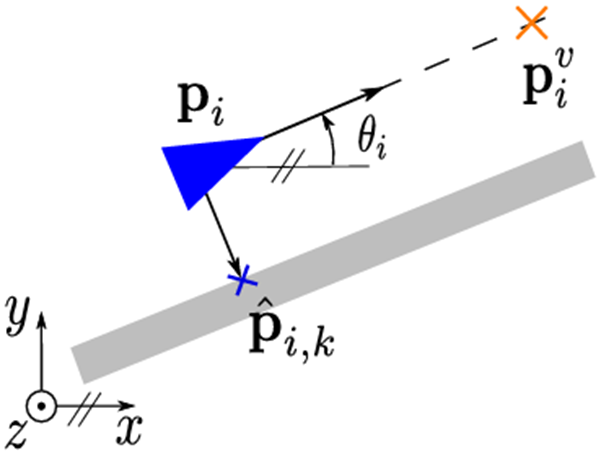
\includegraphics[width=0.25\textwidth]{Pictures/Information about orientation.png}
    \caption{Information about orientation.}
    \label{fig:Information about orientation}
\end{figure}

\begin{figure}[h]
    \centering
    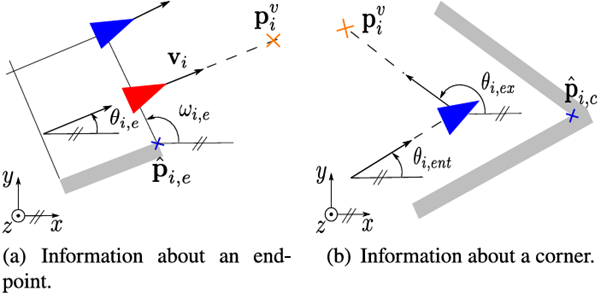
\includegraphics[width=0.4\textwidth]{Pictures/Endpoint and corner Information.png}
    \caption{Endpoint and corner Information.}
    \label{fig:Endpoint and corner Information}
\end{figure}

\begin{table}[h]
\centering
\begin{tabular}{ll}
\hline
\textbf{status$_i$} & \textbf{Definition} \\
\hline
0 & Motion toward the desired goal position \\
1 & Obstacle detection and tangential navigation \\
2 & Handling the endpoint of an obstacle \\
3 & Corner avoidance maneuver \\
4 & Orientation phase \\
5 & Tangential navigation based on received information \\
6 & Waiting mode \\
\hline
\end{tabular}
\caption{Definition of action statuses.}
\label{tab:status}
\end{table}


\section{Collective navigation using shared information}
This section explains how the procedures of a single robot can be extended to a 
multi-robot system. For this purpose, seven \textbf{statuses} are defined in which 
a robot can be found, with each robot starting in \textbf{status 0}.

\subsection*{Collective tangential navigation}
Collective tangential navigation comprises 
\textbf{status 1}, \textbf{4} and \textbf{5}. If a 
robot detects an obstacle within its perception range \( r_{\mathrm{tan}} \), it initiates 
tangential navigation, as with a single robot. This action is referred to as 
\textbf{status 1}. The information obtained in this process is forwarded to neighboring 
robots.
Since the control variable \( u_i^\alpha \) according to equation \eqref{eq:19} can cause robots 
to move away from each other by repelling each other perpendicular to the obstacle, which could unintentionally 
trigger a change from \textbf{status 0} to \textbf{1}, an 
ignorance condition (\eqref{eq:15}) 
was developed so that robots can ignore obstacles.
\begin{equation}
    \begin{split}
    (|\upsilon_i| > 90^\circ \wedge |\beta_i| > 91^\circ) \vee \\
    \| \hat{p}_{i,k} - p_i \| > 0.3 \cdot (r_{\text{tan}} - d_s) + d_s
    \end{split}
    \label{eq:15}
\end{equation}

If new information from the communication network causes a robot to be 
misaligned and the difference between its current movement 
and target orientation is greater than 45°, it switches to 
status 4 to correct its orientation.
If a robot calculates a virtual goal using equation \eqref{eq:37} based on the information 
it has received, it is in \textbf{status 5}.
To prevent robots from detecting obstacle endpoints too late if they have only been detected 
by other neighboring robots, a distance estimation with case differentiation 
(\eqref{eq:40}) is performed.
To prevent robots from detecting obstacle endpoints too late when these have only 
been detected by other neighboring robots, a distance estimation is performed with 
a case distinction (\eqref{eq:30}). This allows the robot to adjust its target orientation timely and thus avoid delays in the movement sequence.

\subsection*{Collective corner avoidance}
If a robot approaches a corner, it can 
navigate around it as described in Section~\ref{sec:Single robot navigation}, 
while also using information from the communication network. 
This action is referred to as \textbf{status 3}.

To ensure that no possible passages 
(e.g., between two obstacles) are overlooked, the robot first checks the 
condition \eqref{eq:39}. Only if this condition is met is the corner recognized as such.
The robot then defines a new virtual goal and switches to \textbf{status 4} 
to realign itself. At the same time, it sends information about the recognized corner 
to the neighboring robots.
However, if the condition \eqref{eq:39} is not met, the robot initially remains in 
waiting state (\textbf{status 6}). In this state, it monitors the communication network 
of its neighbors. If information with \textbf{status 3} or \textbf{4} is classified as relevant,
 the robot adopts it and leaves the waiting state. If, 
instead, there is relevant information with \textbf{status 1} or \textbf{2}, it adapts accordingly 
and either follows the tangential navigation or the maneuver at an obstacle endpoint.

\subsection*{Collective motion at obstacle extremities}
If a robot detects the endpoint of an obstacle, it follows virtual goal positions 
on a circular path (\textbf{status 2}), as described in 
Section~\ref{sec:Single robot navigation}. Each 
robot sets individual targets on this path and shares information about the 
endpoint in its network (Fig.~\ref{fig:Collective maneuver at an obstacle endpoint}).

\begin{figure}[h]
    \centering
    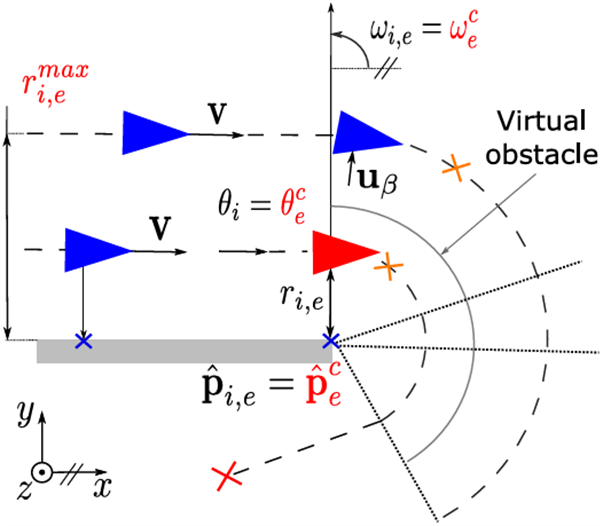
\includegraphics[width=0.4\textwidth]{Pictures/Collective maneuver at an obstacle endpoint.png}
    \caption{Collective maneuver at an obstacle endpoint.}
    \label{fig:Collective maneuver at an obstacle endpoint}
\end{figure}

After receiving the endpoint data, a robot checks its 
position by orthogonal projection onto a virtual start line 
before beginning the circular motion. If the robot has not yet reached this start line 
(\eqref{eq:40}), it sets further tangential targets and adjusts its 
speed to the minimum speed for circular motion 
(\eqref{eq:41} to \eqref{eq:42}). Once it reaches the start line, circular motion begins 
according to the scheme presented in 
Section~\ref{sec:Single robot navigation}.

During the movement, a component from equation \eqref{eq:19} ensures that the robot 
reaches its target on the circular path. If a robot exceeds its 
virtual goal, a new target position is calculated.

The robots move on individual circular paths with 
different radii, which means that inner circles result in shorter paths. 
The speed consensus for circular motion is based on equal 
angular velocities. For this purpose, a minimum angular velocity (\eqref{eq:43}) 
is specified and the control variable from equation \eqref{eq:19} is replaced by an 
adapted control variable 
from equations \eqref{eq:44} and \eqref{eq:45}. 
This allows the robots to circle the end of the obstacle uniformly.

\subsection*{Conditional Braking}
When several robots in a group perform a circular movement around an obstacle, differences in the timing of leaving the circular path can cause speed differences that lead to the group breaking apart.
To prevent this, robots that have already passed the obstacle are slowed down.
This deceleration remains active until the last robot in the group has left the circular path.
To determine this last robot, a new coordinate system is defined whose origin lies at the end point of the obstacle. In this system, the 
position of each robot is projected onto the x-axis. Using these projected 
positions and equation \eqref{eq:46}, the robots observe their neighborhood and 
identify the robot that is furthest behind.

Via gossip-like 
communication\footnote{local, decentralized, and iterative information exchange}, the entire group is informed about this candidate until 
all robots have determined the global rear robot. Once 
this robot has completed its circular movement, it sends a reset signal to 
release the brakes of the remaining robots and resynchronize the group movement.

\subsection*{Watchdog timer}
If the speed of a robot falls below a defined threshold value, 
it activates a self-monitoring mechanism called the \textit{watchdog timer}. 
The robot stores its current position and the current time. 
The timer is deactivated again as soon as the robot moves more than a specified threshold 
value within the following time steps 
(the robot assumes that it has left a possible deadlock\footnote{no-exit situation}). 
However, if the robot hardly moves for a period of 15 seconds 
and the timer has not been deactivated, it automatically switches to \textbf{status 0} 
and moves toward the desired goal. Although this measure can lead to 
fragmentation of the group, it ensures that each robot 
reaches the desired goal.


\section{Simulation results}
The simulation results are presented using two scenarios: 
one with a zigzag obstacle and one with a corridor with obstacles. 
In both cases, twelve robots are randomly 
positioned within a starting area, each without initial velocity. 
In addition, a desired goal (marked with a red cross) is defined.

The robots are represented as black triangles in the figures. 
Their movement is visualized by a colored line behind the triangles, 
with the direction of movement corresponding to the orientation of the triangle's tip. The black 
lines between the robots indicate the active communication network. 
The figures show snapshots at specific points in time or 
relevant events during the simulation.

In the first scenario (Fig.~\ref{fig:Sequential snapshots of 12 robots collectively navigating through a zigzag obstacle}), the following sequences are shown:
\begin{itemize}
\item (a): Detection of an obstacle and start of tangential navigation.
\item (b): Detection of a corner point and execution of the corner avoidance maneuver.
\item (c) and (d): Detection of an end point and initiation of circular movement around the obstacle.
\item (e): Approximation of the robots to the obstacle to optimize navigation using equation \eqref{eq:46}.
\item (f): Reaching the desired goal.
\end{itemize}

The same procedures are used in the second corridor scenario (Fig.~\ref{fig:Sequential snapshots of 12 robots collectively navigating through a corridor}).

\subsection*{Guideline for parameter choice}
The parameters of the relevance equation \eqref{eq:11} should be selected depending on the 
respective scenario. A global behavior of the 
multi-robot system, in which all robots perform identical actions almost simultaneously,
 is suitable for smaller systems with six to twelve 
robots if their distribution in relation to the obstacles 
is low. In this case, the relevance of the time of the information package 
($\mathrm{rel}_{\mathrm{t}}$) and the relevance of the action status ($\mathrm{rel}_{\mathrm{type}}$) should be weighted higher 
than the other values so that robots react uniformly and as synchronously as possible
to current events in the communication network.

However, with an increasing number of robots or a denser obstacle constellation, 
such global behavior can be problematic, as individual 
robots could receive several relevant information packages at the same time. 
In these situations, robots should pay more attention to their own position and local 
information. To this end, the relevance of the distance to the obstacle 
($\mathrm{rel}_{\mathrm{dist}}$), the relevance of the expected orientation for the next action 
($\mathrm{rel}_{\mathrm{exp}}$) and the relevance of the sender of the information ($\mathrm{rel}_{\mathrm{o}}$) 
are weighted more heavily than $\mathrm{rel}_{\mathrm{t}}$ and $\mathrm{rel}_{\mathrm{type}}$.

The effects of these different weightings are shown in the following figures:
\begin{itemize}
\item Fig.~\ref{fig:Sequential snapshots of 20 robots collectively navigating around two 
circular obstacles} 
shows a \textit{squeezing maneuver} in which the 
group of robots move between two circular obstacles.
\item Fig.~\ref{fig:Sequential snapshots of 20 robots collectively navigating around a 
semi circular obstacle} 
shows how a semicircular obstacle 
divides the group. The robots then correct their direction of movement 
by checking and adjusting their current action statuses.
\item Fig.~\ref{fig:Sequential snapshots of 20 robots collectively navigating around 
small circular obstacles} illustrates that prioritized 
obstacle avoidance causes fragmentation of the group. 
Nevertheless, all robots ultimately reach the desired destination.
\end{itemize}


\section{Conclusion}
In this work, a method for collective navigation of autonomous robots in unknown environments 
was developed. The approach combines a tangential navigation strategy with the exchange of local 
environmental information via a communication network. Collision-free and coordinated movements 
of the robots are enabled by virtual potential field-based forces that generate swarm-like behavior. 
Targeted adjustment of the relevance equation parameters and weighting can prevent fragmentation 
of the group. Individual robots retain the ability to reach their destination even without 
group connection. For robots whose position can be changed independently of their orientation, a sufficiently large safety distance and reduced speed are particularly crucial. 
Future work will address real-time implementation, optimization of wireless communication, 
and alternative network structures for the robots.


\section*{Appendix}

\subsection*{Equations and conditions}
\begin{equation}
\| z \|_{\sigma} = \frac{1}{\epsilon} \left( \sqrt{1 + \epsilon \| z \|^2} - 1 \right)
\label{eq:16}
\end{equation}
A modified distance measure called the $\sigma$-norm is introduced to ensure differentiability at zero and improve stability at small inter-agent distances.

\begin{equation}
\rho_h(z) =
\begin{cases}
1, & z \in [0, h) \\
\frac{1}{2} \left( 1 + \cos \left( \pi \frac{z - h}{1 - h} \right) \right), & z \in [h, 1) \\
0, & \text{otherwise}
\end{cases}
\label{eq:17}
\end{equation}
A smooth transition equation is defined to weight the influence of neighboring agents based on their relative distances.

\begin{equation}
a_{ij}(p) = \rho_h \left( \frac{\| p_j - p_i \|_{\sigma}}{r^{\alpha}} \right), \quad j \neq i
\label{eq:18}
\end{equation}
The adjacency matrix element $a_{ij}$ quantifies how strongly agent $j$ influences agent $i$ based on their distance.

\begin{equation}
u^{\alpha}_i = c_{\alpha 1} \sum_{j \in N^{\alpha}_i} \phi^{\alpha} \left( \| p_j - p_i \|_{\sigma} \right) n_{ij}
+ c_{\alpha 2} \sum_{j \in N^{\alpha}_i} a_{ij}(p) (v_j - v_i)
\label{eq:19}
\end{equation}
The control input for flock-like behavior consists of a gradient-based term for cohesion/separation and a consensus term for velocity alignment.

\begin{equation}
\phi^{\alpha}(z) = \rho^{\alpha}_h \left( \frac{z}{r^{\alpha}} \right) \varphi(z - d^{\alpha})
\label{eq:20}
\end{equation}
This equation modulates the inter-agent force depending on the distance and neighborhood weight.

\begin{equation}
\varphi(z) = \frac{1}{2} \left( (a + b) \sigma_1(z + c) + (a - b) \right)
\label{eq:21}
\end{equation}
An uneven sigmoid equation $\varphi(z)$ is used to create asymmetric attraction and repulsion behaviors between agents.

\begin{equation}
N^{\beta}_i = \left\{ \hat{p}_{i,k} \;\big|\; \| \hat{p}_{i,k} - p_i \| < r_s \right\}
\label{eq:22}
\end{equation}
The set $N^{\beta}_i$ represents all detected obstacle points within the sensing range of agent $i$.

\begin{equation}
u^{\beta}_i = c_{\beta 1} \sum_{k \in N^{\beta}_i} \phi^{\beta} \left( \| \hat{p}_{i,k} - p_i \|_{\sigma} \right) \hat{n}_{i,k}
+ c_{\beta 2} \sum_{k \in N^{\beta}_i} b_{i,k}(p) (\hat{v}_{i,k} - v_i)
\label{eq:23}
\end{equation}
The control input $u^{\beta}_i$ generates repulsive forces to avoid obstacles based on their distance and motion relative to the agent.

\begin{equation}
\phi^{\beta}(z) = \rho^{\beta}_h \left( \frac{z}{d^{\beta}} \right) \left( \sigma_1(z - d^{\beta}) - 1 \right)
\label{eq:24}
\end{equation}
This equation defines a repulsive force magnitude depending on the distance to the obstacle.

\begin{equation}
u^{\gamma}_i = -c_{\gamma 1} \, \sigma_1(p_i - p_d) - c_{\gamma 2} \, v_i
\label{eq:25}
\end{equation}
The navigation input $u^{\gamma}_i$ guides the agent toward the desired goal position while damping its velocity.

\begin{equation}
\gamma_i =
\begin{cases}
\beta_i - \alpha_i - 90^\circ, & \text{if } \beta_i \geq 0^\circ \\
\beta_i - \alpha_i + 90^\circ, & \text{if } \beta_i < 0^\circ
\end{cases}
\label{eq:26}
\end{equation}
The rotation angle $\gamma_i$ is computed based on the relative position of the obstacle and the desired goal, depending on the obstacle’s side.

\begin{equation}
c_r =
\begin{cases}
-1, & \text{for clockwise rotation} \\
1,  & \text{for counter-clockwise rotation}
\end{cases}
\label{eq:27}
\end{equation}
The constant $c_r$ determines the predefined direction of rotation: clockwise or counter-clockwise.

\begin{equation}
\gamma_i = \beta_i - \alpha_i + c_r \cdot 90^\circ
\label{eq:28}
\end{equation}
The rotation angle $\gamma_i$ is modified using the predefined rotation direction $c_r$.

\begin{equation}
p^{v}_i = p_i +
\begin{pmatrix}
\cos(\gamma_i) & -\sin(\gamma_i) \\
\sin(\gamma_i) & \cos(\gamma_i)
\end{pmatrix}
(p_d - p_i)
\label{eq:29}
\end{equation}
The virtual goal position $p^v_i$ is calculated by rotating the vector toward the goal by angle $\gamma_i$.

\begin{equation}
u^{\gamma}_i = -c_{\gamma 1} \cdot \left( c_n \cdot \frac{p_i - p^v_i}{\| p_i - p^v_i \|} \right) - c_{\gamma 2} \, v_i
\label{eq:30}
\end{equation}
The navigation control input $u^{\gamma}_i$ drives the agent toward the virtual goal position with controlled acceleration.

\begin{equation}
\gamma_i =
\begin{cases}
\beta_i - \alpha_i - \tau_i, & \text{if } \epsilon_i \geq 0^\circ \\
\beta_i - \alpha_i + \tau_i, & \text{if } \epsilon_i < 0^\circ
\end{cases}
\label{eq:31}
\end{equation}
The angle $\gamma_i$ defines the rotation required to generate a temporary goal during corner avoidance, depending on the obstacle configuration.

\begin{equation}
\tau_i = | \epsilon_i | + 90^\circ
\label{eq:32}
\end{equation}
The auxiliary angle $\tau_i$ determines the required deviation angle in a corner, based on the angle $\epsilon_i$ between obstacle edges.

\begin{equation}
p^v_i = p_i +
\begin{pmatrix}
\cos(\gamma_i) & -\sin(\gamma_i) \\
\sin(\gamma_i) & \cos(\gamma_i)
\end{pmatrix}
\begin{pmatrix}
0.5 \cdot d_s \cdot \cos(\theta^d_i) \\
0.5 \cdot d_s \cdot \sin(\theta^d_i)
\end{pmatrix}
\label{eq:33}
\end{equation}
The virtual goal $p^v_i$ is defined for precise corner maneuvers and is located relative to the current position and desired direction.

\begin{equation}
\gamma_i =
\begin{cases}
+\delta, & \text{if } \beta_{i,e} \geq 0^\circ \\
-\delta, & \text{if } \beta_{i,e} < 0^\circ
\end{cases}
\label{eq:34}
\end{equation}
The rotation angle $\gamma_i$ is determined based on the obstacle endpoint configuration and whether the obstacle lies to the left or right.

\begin{equation}
p^v_i = \hat{p}_{i,e} +
\begin{pmatrix}
\cos(\gamma_i) & -\sin(\gamma_i) \\
\sin(\gamma_i) & \cos(\gamma_i)
\end{pmatrix}
n_{i,e}
\label{eq:35}
\end{equation}
The virtual goal $p^v_i$ is calculated around the last detected obstacle point $\hat{p}_{i,e}$ along a circular path.

\begin{equation}
| \alpha_i | \leq \delta
\label{eq:36}
\end{equation}
The robot leaves the circular path when its orientation to the goal satisfies this condition.

\begin{equation}
p^v_i = p_i +
\begin{pmatrix}
\cos(\theta^c) & -\sin(\theta^c) \\
\sin(\theta^c) & \cos(\theta^c)
\end{pmatrix}
\cdot e_x \cdot s
\label{eq:37}
\end{equation}
A virtual goal $p^v_i$ is created based on a communicated orientation angle $\theta^c$, used during tangential navigation by information sharing.

\begin{equation}
\theta_i(t_{k+1}) =
\begin{cases}
\theta^c - 20^\circ, & \text{if } \| \tilde{p}_{i,k} - p_i \| < 1.5 \cdot r \wedge \beta_i < 0^\circ \\
\theta^c + 20^\circ, & \text{if } \| \tilde{p}_{i,k} - p_i \| < 1.5 \cdot r \wedge \beta_i \geq 0^\circ
\end{cases}
\label{eq:38}
\end{equation}
The angle $\theta_i(t_{k+1})$ is adjusted to anticipate obstacle endpoints by modifying the goal orientation based on the relative obstacle side.

\begin{equation}
\| \tilde{p}_{i,k} - p_i \| < 3 \cdot d_s \wedge \| \tilde{p}_{i,k} - \hat{p}^c_k \| < 3 \cdot d_s
\label{eq:39}
\end{equation}
This condition is used to detect a corner configuration based on the distances between the projected point and obstacle references.

\begin{equation}
( p^*_i - p_i ) = -k \cdot ( p^v_i - p_i )
\label{eq:40}
\end{equation}
This equation checks whether the agent has reached the start line for initiating a circular motion around an obstacle.

\begin{equation}
v^{\text{ref}}_i = \frac{p^v_i - p_i}{\| p^v_i - p_i \|} \cdot \frac{d_s}{r^{\text{max}}_{i,e}} \cdot v_{\text{max}}
\label{eq:41}
\end{equation}
The reference velocity $v^{\text{ref}}_i$ is calculated to control the agent’s speed proportionally to its distance from the obstacle.

\begin{equation}
u^{\gamma}_{i,e} = -c_{\gamma e} ( v_i - v^{\text{ref}}_i )
\label{eq:42}
\end{equation}
The control input $u^{\gamma}_{i,e}$ guides the agent toward the virtual goal with speed matching the reference velocity.

\begin{equation}
\omega_{\text{min}} = \frac{v_{\text{max}}}{r^{\text{max}}_{i,e}}
\label{eq:43}
\end{equation}
The minimum angular velocity $\omega_{\text{min}}$ is computed to achieve synchronized circular motion with the largest turning radius.

\begin{equation}
v^{\text{ref}}_i = \frac{p^v_i - p_i}{\| p^v_i - p_i \|} \cdot \omega_{\text{min}} \cdot r_{i,e}
\label{eq:44}
\end{equation}
The reference velocity $v^{\text{ref}}_i$ is computed to ensure angular velocity consensus during the circular maneuver.

\begin{equation}
u^{\gamma}_{i,e} = -c_{\gamma e} ( v_i - v^{\text{ref}}_i )
\label{eq:45}
\end{equation}
The control input $u^{\gamma}_{i,e}$ ensures convergence to the reference velocity for synchronized circular motion.

\begin{equation}
d(i) =
\begin{cases}
\| p_{i,E} - 0_E \|, & \text{wenn } (p_{i,E} - 0_E) = k \cdot e_x^E \\
-\| p_{i,E} - 0_E \|, & \text{wenn } (p_{i,E} - 0_E) = -k \cdot e_x^E
\end{cases}
\label{eq:46}
\end{equation}
This equation defines the position of an agent projected onto a coordinate axis, used to identify the backmost agent in the group.

\subsection*{Figures and tables}
\begin{figure*}[htbp]
    \centering
    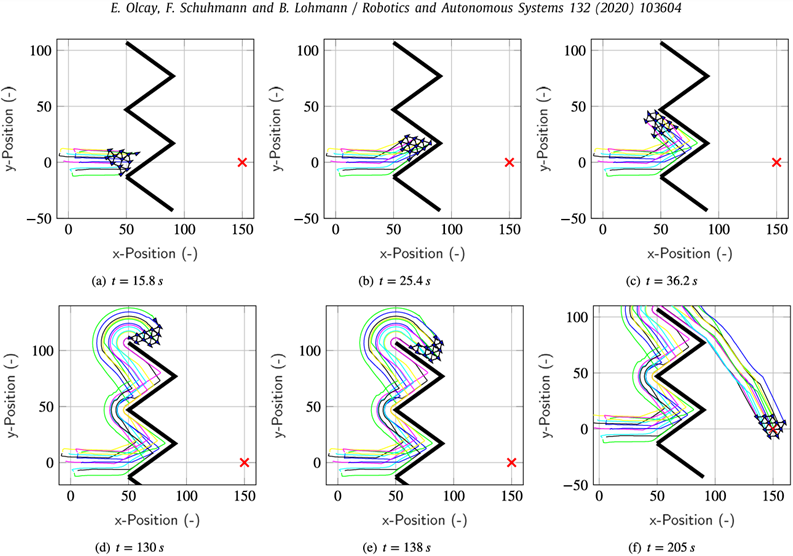
\includegraphics[width=0.8\textwidth]{Pictures/Sequential snapshots of 12 robots collectively navigating through a zigzag obstacle.png}
    \caption{Sequential snapshots of 12 robots collectively navigating through a zigzag obstacle.}
    \label{fig:Sequential snapshots of 12 robots collectively navigating through a zigzag obstacle}
\end{figure*}
\begin{figure*}[htbp]
    \centering
    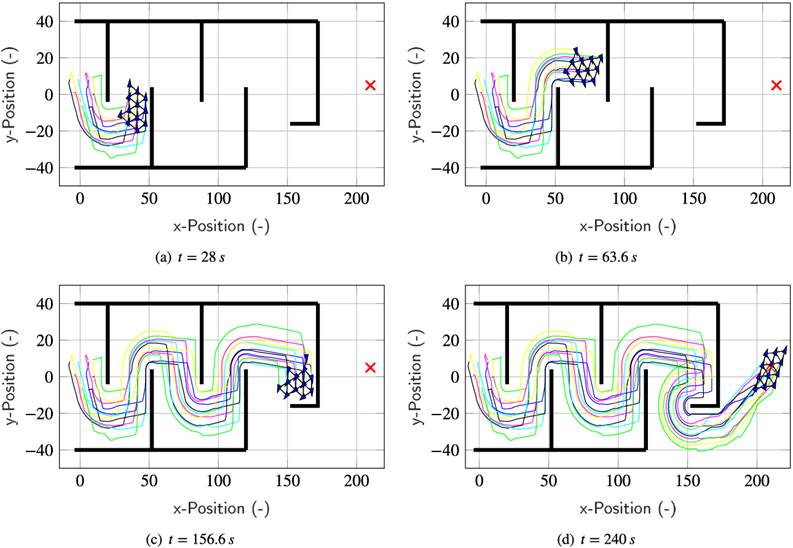
\includegraphics[width=0.8\textwidth]{Pictures/Sequential snapshots of 12 robots collectively navigating through a corridor.png}
    \caption{Sequential snapshots of 12 robots collectively navigating through a corridor.}
    \label{fig:Sequential snapshots of 12 robots collectively navigating through a corridor}
\end{figure*}
\begin{figure*}[htbp]
    \centering
    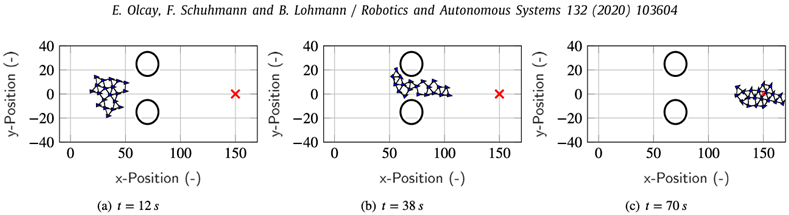
\includegraphics[width=0.8\textwidth]{Pictures/Sequential snapshots of 20 robots collectively navigating around two circular obstacles.png}
    \caption{Sequential snapshots of 20 robots collectively navigating around two circular obstacles.}
    \label{fig:Sequential snapshots of 20 robots collectively navigating around two circular obstacles}
\end{figure*}
\begin{figure*}[htbp]
    \centering
    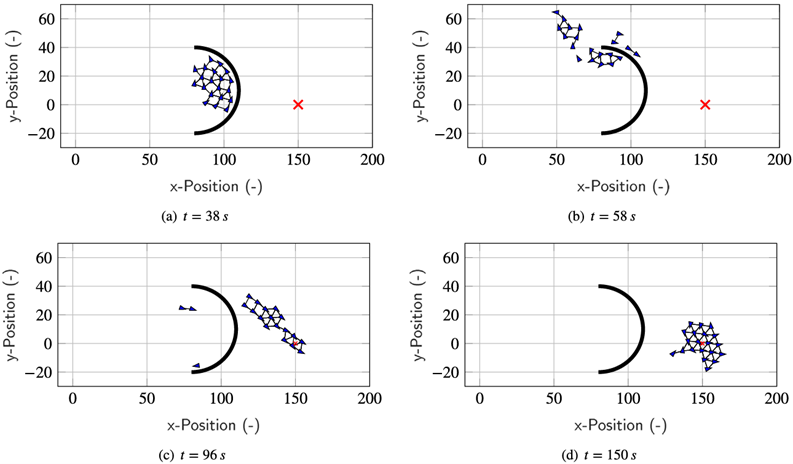
\includegraphics[width=0.8\textwidth]{Pictures/Sequential snapshots of 20 robots collectively navigating around a semi circular obstacle.png}
    \caption{Sequential snapshots of 20 robots collectively navigating around a semi circular obstacle.}
    \label{fig:Sequential snapshots of 20 robots collectively navigating around a semi circular obstacle}
\end{figure*}
\begin{figure*}[htbp]
    \centering
    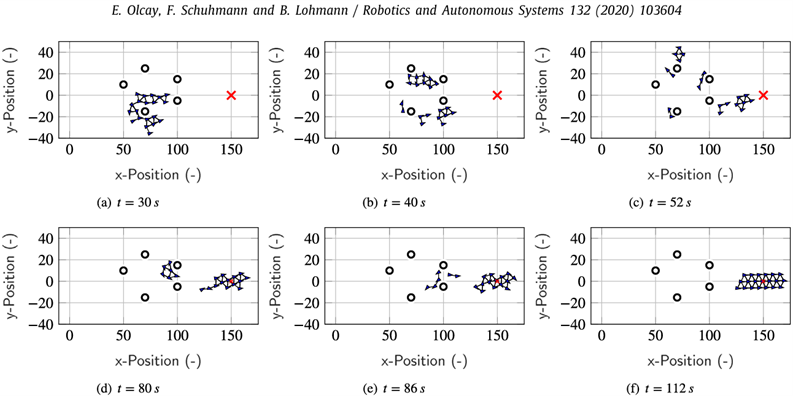
\includegraphics[width=0.8\textwidth]{Pictures/Sequential snapshots of 20 robots collectively navigating around small circular obstacles.png}
    \caption{Sequential snapshots of 20 robots collectively navigating around small circular obstacles.}
    \label{fig:Sequential snapshots of 20 robots collectively navigating around small circular obstacles}
\end{figure*}

\clearpage
\bibliographystyle{IEEEtran}
\bibliography{IEEEabrv,literature}

\end{document}
